\subsection{Large scale simulations}
\label{sec:largescale}

%To check validity of the small-scale experiment results, we performed a larger-scale evaluation based on a modified version of 

Next, our goal is to understand the behavior of our mitigation strategies when deployed on a large-scale real network topology. Our ISP topology is based on a modified version of Rocketfuel's AT\&T topology~\cite{rocketfuel}.
%In order to approximate the general structure of the Internet,
% (scale-free structure, customer-provider, and peer-to-peer relations)
We extract the largest connected component comprising of 562 nodes from this original topology and separate the nodes into three categories: clients, gateways, and backbones. Nodes having degree than four are classified as clients (344 red nodes as shown in Fig.~\ref{fig:large-scale}), nodes directly connected to clients are classified as gateways (109 green nodes), and the remaining nodes as classified as backbones (109 blue nodes). 
%(To ensure that paths in the topology are ``valley-free,'' we augmented the topology with necessary backbone-to-backbone links.) 
We assign bandwidth and  delay values to links based on their type---both values are random numbers within the respective ranges as shown in Table~\ref{tab:large-scale}. We experiment with placing the data producer at both a gateway node as well as backbone node, which we randomly pick for each simulation run. Similar to the binary tree topology experiments, we fix the number of malicious nodes at approximately 40\% (140 out of 344 client nodes in the topology) and randomly pick these nodes for each simulation run. We conduct 10 simulation runs for each mitigation algorithm, with the attack duration spanning a 5 minute interval.

\begin{figure}[htbp]
  \centering
  \vspace{-.1cm}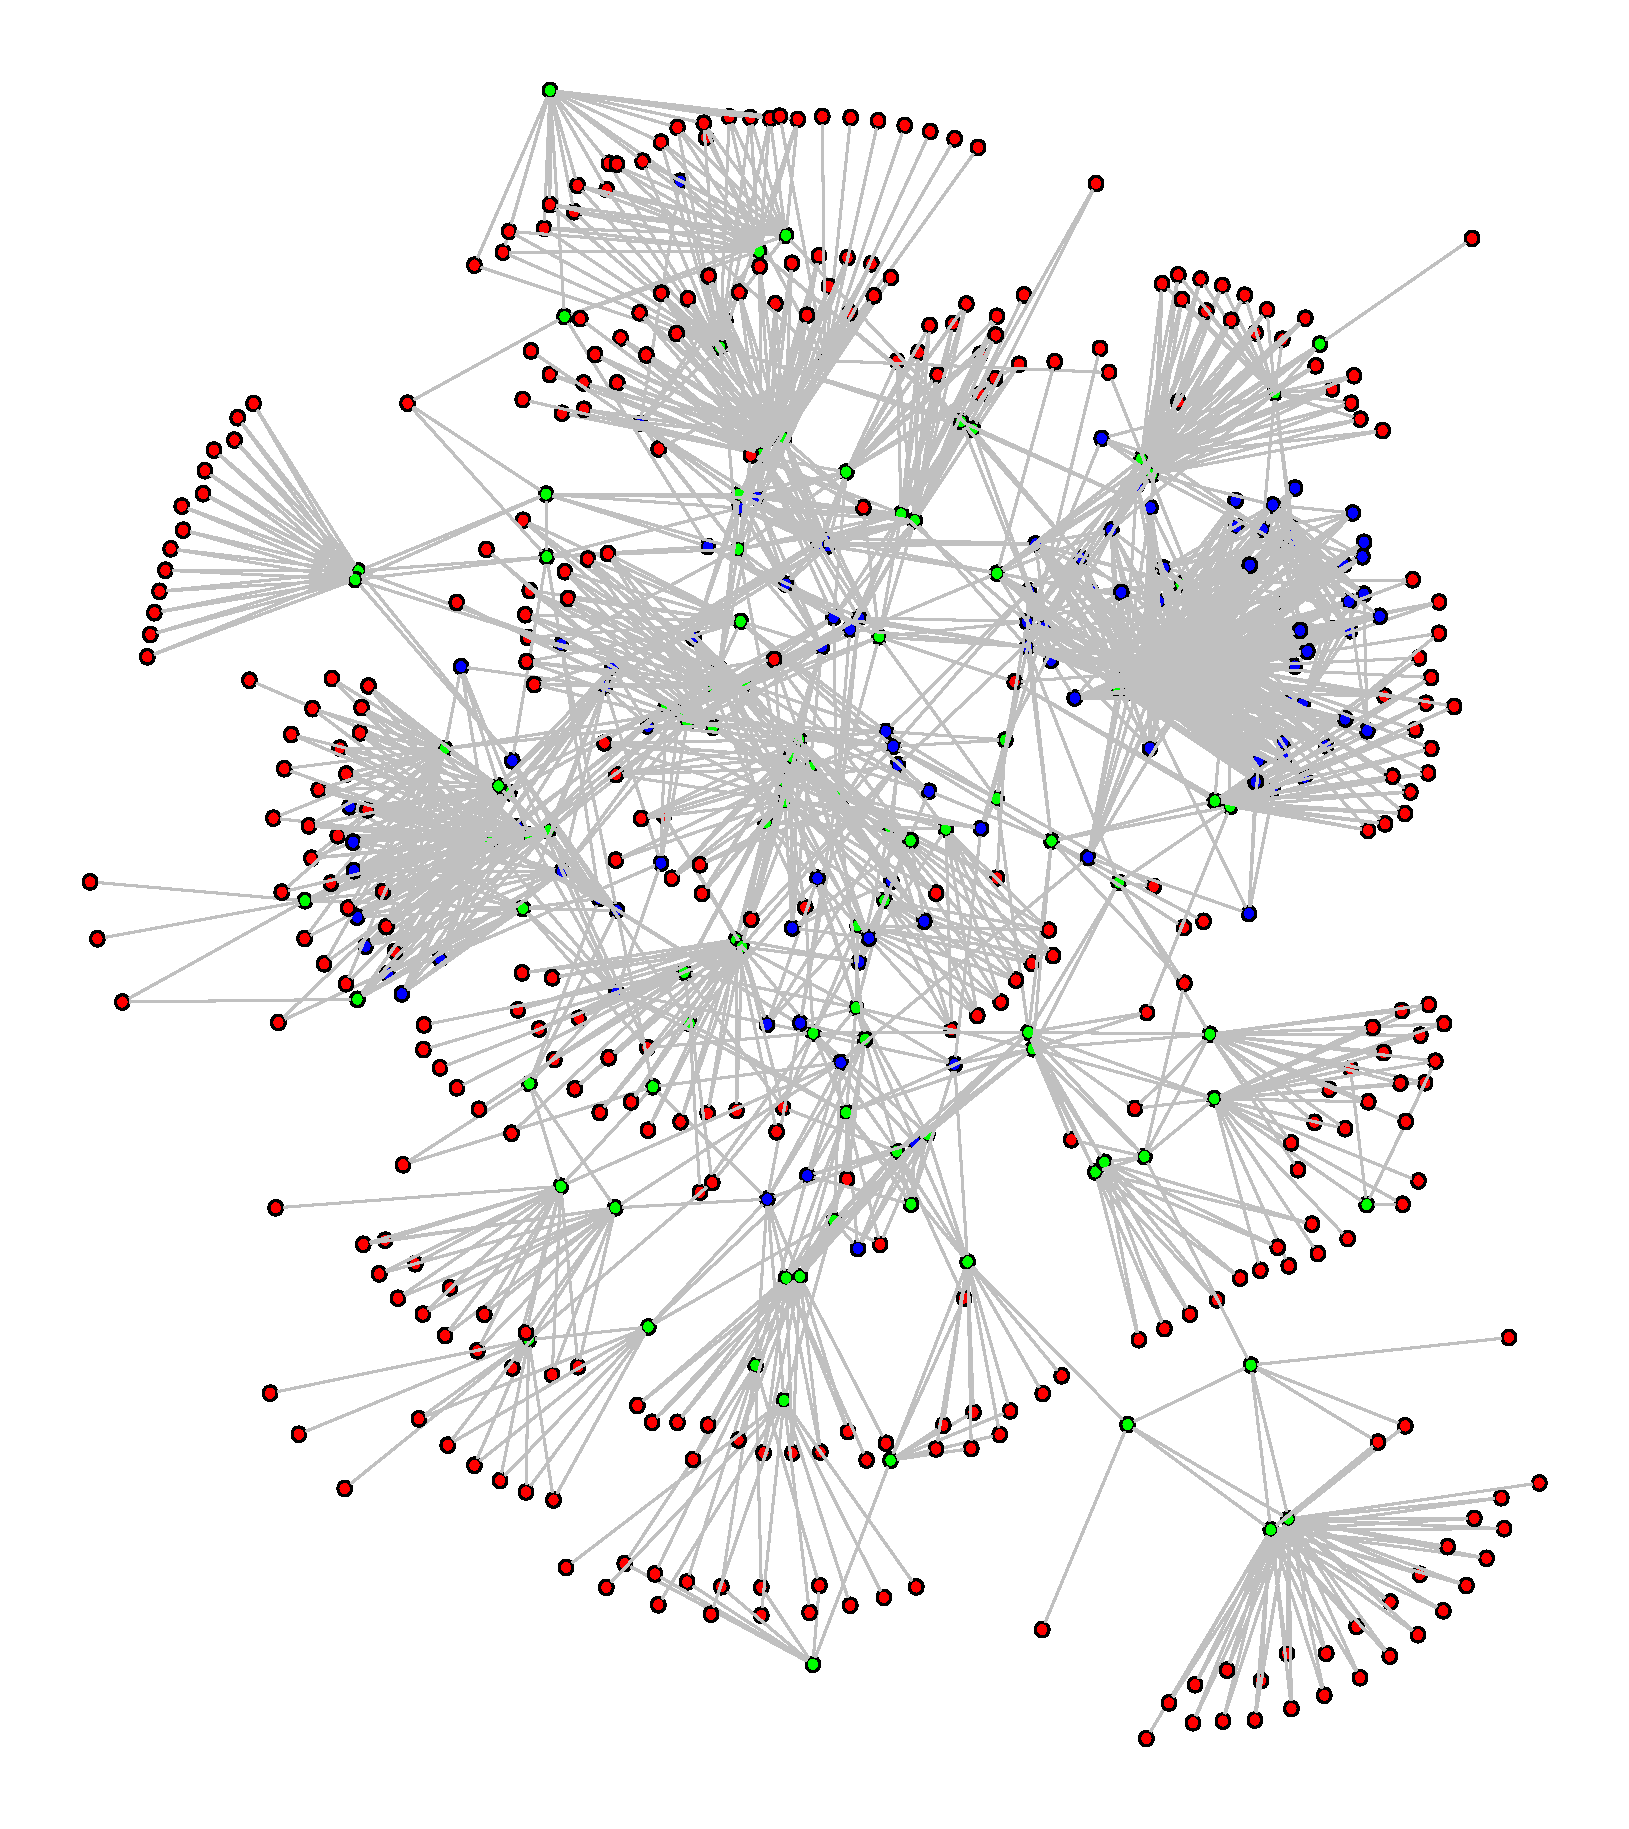
\includegraphics[scale=0.15,angle=90]{7018-r0}
  \caption{Internet-like topology: 344 client routers (red), 109 gateway routers (green), 109 backbone routers (blue)}\vspace{-.2cm}
  \label{fig:large-scale-topo}
\end{figure}

\begin{table}[htbp]
\centering
\caption{Large-scale topology link bandwidth and delay ranges}
\label{tab:large-scale}
\begin{tabular}{|l||c|c||c|c|}
  \hline
  \multirow{2}{*}{\bf Link type} &  \multicolumn{2}{|c||}{\bf Delay} &  \multicolumn{2}{|c|}{\bf Bandwidth} \tabularnewline
  \cline{2-5}
                        &  Min & Max                       &  Min & Max \tabularnewline
  \hline \hline
  Backbone--Backbone    & 5~ms & 10~ms   & 40~Mbps & 100~Mbps \tabularnewline
  \hline
  Gateway--Backbone,    & \multirow{2}{*}{5~ms} & \multirow{2}{*}{10~ms}   
                        & \multirow{2}{*}{10~Mbps} & \multirow{2}{*}{20~Mbps} \tabularnewline
  Gateway--Gateway      & & & & \\
  \hline
  Client--Gateway       & 10~ms & 70~ms   & 1~Mbps  & 3~Mbps \\
  \hline

\end{tabular}
\end{table}

%Priya: Leaving out this in the interest of space...
%Topological location of the data producer plays a key role in its resilience to Interest flooding attacks. For a data producer that %is connected to a client node via a low-bandwidth link, even a small number of junk Interests can impact services for legitimate %users. For a producer located at the backbone with rich connectivity through many high-bandwidth links, an attack might not %be as severe as a majority of legitimate users might not be on the attack path. 


% The results for all attack mitigation algorithms and all runs are aggregated in Fig.~\ref{fig:small-scale attack progress}, where Y-axis represents a minimum and maximum range for observed Interest satisfaction percentages among all nodes and all simulation runs.
% A short and simplistic summary of the results is that the first two attack mitigation methods do not work at all, and the last two are working quite good.

In Fig.~\ref{fig:large-scale}, we summarize our results aggregated over 10 simulations runs for each mitigation algorithm for the scenario where the data producer is placed at a gateway node. We observe similar results for the data producer placed at the backbone node as well. As in the case of the binary-tree topology experiments, token bucket with per interface fairness is the most ineffective algorithm and satisfaction-based pushback is the most effective one.   Interest satisfaction percentage for legitimate users are approximately 25\% and almost 100\% respectively for these two mitigation methodologies.

%
%The evaluation results,\footnote{Note that for larger-scale experiments we reduced attack window to 15~minutes} summarized in Fig.~\ref{fig:large-scale}, show that performance of the token bucket with per interface fairness and satisfaction-based pushback algorithms are about at the same level as in small-scale evaluations (Fig.~\ref{fig:small-scale}), but with larger variations of minimum and maximum instantaneous satisfaction rates.

\begin{figure}[tbh]
 \centering
 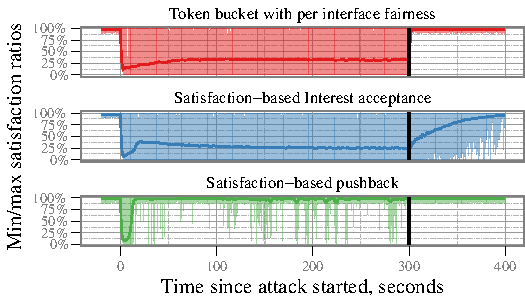
\includegraphics[scale=0.8]{paper-topo-7018-gw/7018-r0-good-0-producer-gw}
 \vspace{-.7cm}\caption{Satisfaction ratio dynamics during the attack for large-scale topology with 40\% attackers)}\vspace{-.4cm}
 % producer on a gateway node
 \label{fig:large-scale}
\end{figure}

Satisfaction-based Interest acceptance algorithm, which was very effective for binary-tree topology, is completely ineffective when deployed in a larger realistic topology. For the duration of the attack, legitimate users experience poor quality of service with only 25\% of their Interests being satisfied and continue to experience degraded service long after the attack has stopped. This poor performance, as detailed in  in Section~\ref{sec:probabilistic}, is due to the fact that each router in the path makes an independent, uncoordinated decision on whether to forward or drop an Interest. In the case of the larger-topology, with much higher average hop count, Interest packets from legitimate users have a very low probability of reaching the data producer, resulting in poor Interest satisfaction statistics, which in turn leads to further penalization of new Interests from them.

To summarize, in all of our simulations, the satisfaction-based pushback algorithm is the most effective technique as it restricts malicious Interests from even entering the network. 
%The only short periods of time when malicious Interests are getting admitted to the network is when routers have either no prior knowledge about per-interface satisfaction ratios (the initial period of the attack) or such knowledge becomes stale (statistics decaying during the attack). As soon as the knowledge is obtained or refreshed, the service for legitimate users returns to norm.


% Alex: Anything else here?

% Alex: I also experimented with placing producer at the backbone, getting slightly better results for all algorithms.  Though I'm not sure there is any value to put those results in the paper


%%% Local Variables: 
%%% mode: latex
%%% TeX-master: "paper"
%%% End: 
